% Individual LaTeX Figure Code Snippets
% Copy and paste any of these figures into your Overleaf project

\documentclass{article}
\usepackage{pgfplots}
\usepackage{subcaption}
\usepackage{graphicx}
\usepackage{geometry}
\usepackage{float}
\usepackage{xcolor}
\usepackage{amsmath}
\usepackage{caption}

\geometry{a4paper, margin=1in}

\pgfplotsset{
    compat=1.17,
    grid style={dashed, gray!30},
    every axis/.append style={
        thick,
        font=\small
    },
    every axis title/.append style={font=\bfseries\large},
    every axis label/.append style={font=\bfseries},
    legend style={
        at={(0.98,0.98)},
        anchor=north east,
        font=\small
    }
}

\definecolor{cfoBlue}{HTML}{2E86AB}
\definecolor{krumOrange}{HTML}{F18F01}
\definecolor{trimmedRed}{HTML}{C73E1D}
\definecolor{medianGreen}{HTML}{6A994E}
\definecolor{trustPurple}{HTML}{A23B72}
\definecolor{bulyanBrown}{HTML}{BC4B51}

\begin{document}

% Figure 1: Traditional BFT Comparison
\begin{figure}[H]
\centering
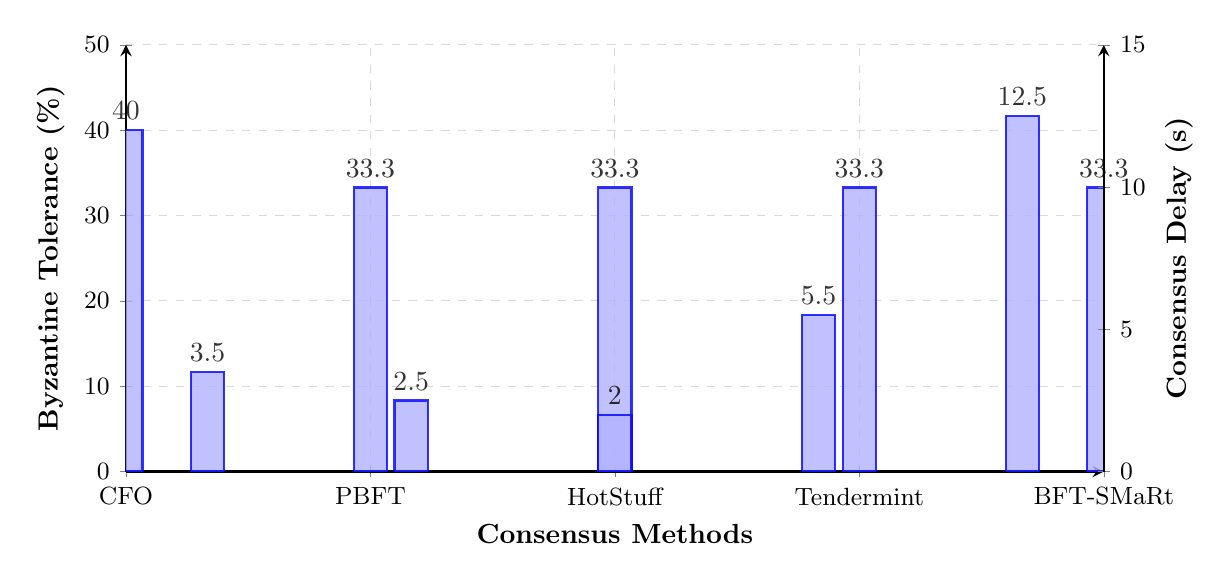
\begin{tikzpicture}
\begin{axis}[
    width=14cm,
    height=7cm,
    ybar=5pt,
    bar width=12pt,
    symbolic x coords={CFO,PBFT,HotStuff,Tendermint,BFT-SMaRt},
    xtick=data,
    ylabel={Byzantine Tolerance (\%)},
    xlabel={Consensus Methods},
    ymin=0, ymax=50,
    grid=both,
    grid style={dashed, gray!30},
    axis lines=left,
    axis line style={thick},
    every axis plot/.append style={fill=cfoBlue, opacity=0.8},
    nodes near coords,
    nodes near coords align={above},
    every node near coord/.append style={font=\bfseries, color=black}
]

\addplot coordinates {
    (CFO,40)
    (PBFT,33.3)
    (HotStuff,33.3)
    (Tendermint,33.3)
    (BFT-SMaRt,33.3)
};

\end{axis}

\begin{axis}[
    width=14cm,
    height=7cm,
    ybar=5pt,
    bar width=12pt,
    symbolic x coords={CFO,PBFT,HotStuff,Tendermint,BFT-SMaRt},
    xtick=data,
    ylabel={Consensus Delay (s)},
    ymin=0, ymax=15,
    axis y line=right,
    axis x line=none,
    every axis plot/.append style={fill=trustPurple, opacity=0.8},
    nodes near coords,
    nodes near coords align={above},
    every node near coord/.append style={font=\bfseries, color=black}
]

\addplot coordinates {
    (CFO,3.5)
    (PBFT,2.5)
    (HotStuff,2)
    (Tendermint,5.5)
    (BFT-SMaRt,12.5)
};

\end{axis}
\end{tikzpicture}
\caption{Comparison with Traditional BFT Consensus Algorithms}
\end{figure}

% Figure 2: Federated Learning Comparison
\begin{figure}[H]
\centering
\begin{subfigure}{0.48\textwidth}
\centering
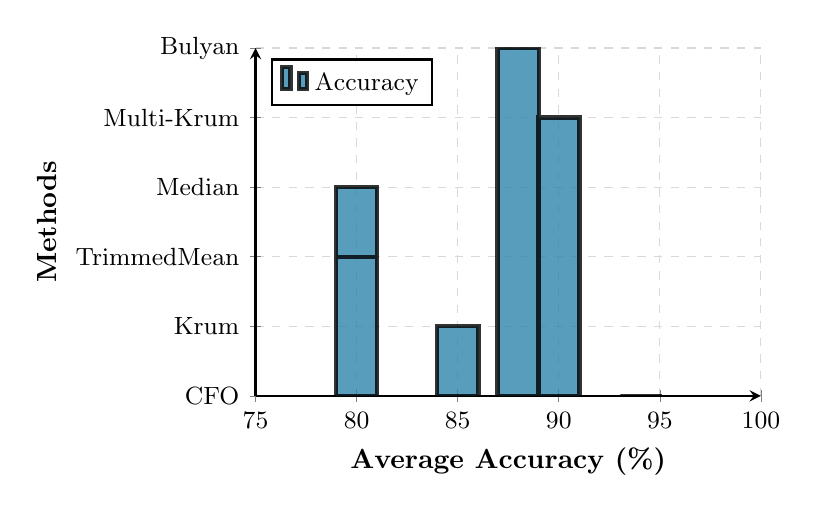
\begin{tikzpicture}
\begin{axis}[
    width=8cm,
    height=6cm,
    ybar,
    bar width=15pt,
    symbolic y coords={CFO,Krum,Trimmed\\Mean,Median,Multi-Krum,Bulyan},
    ytick=data,
    xlabel={Average Accuracy (\%)},
    ylabel={Methods},
    xmin=75, xmax=100,
    grid=both,
    grid style={dashed, gray!30},
    axis lines=left,
    axis line style={thick},
    legend pos=north west
]

\addplot[fill=cfoBlue, opacity=0.8, draw=black, line width=1.5pt] coordinates {
    (94.08,CFO)
    (85,Krum)
    (80,Trimmed\\Mean)
    (80,Median)
    (90,Multi-Krum)
    (88,Bulyan)
};

\legend{Accuracy}

\end{axis}
\end{tikzpicture}
\caption{Prediction Accuracy Comparison}
\end{subfigure}
\hfill
\begin{subfigure}{0.48\textwidth}
\centering
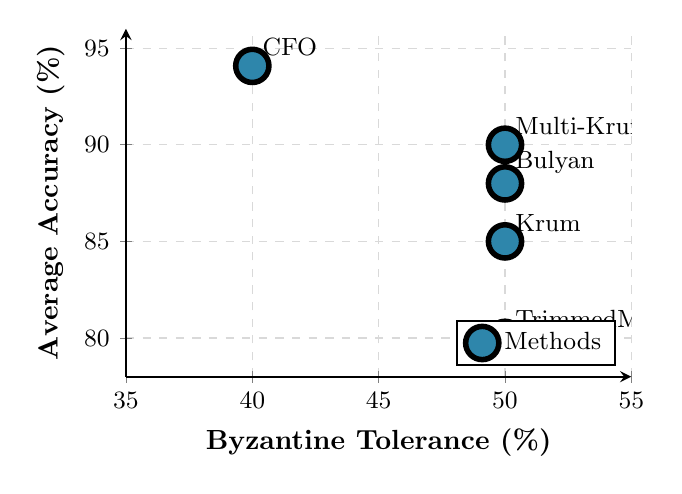
\begin{tikzpicture}
\begin{axis}[
    width=8cm,
    height=6cm,
    xlabel={Byzantine Tolerance (\%)},
    ylabel={Average Accuracy (\%)},
    xmin=35, xmax=55,
    ymin=78, ymax=96,
    grid=both,
    grid style={dashed, gray!30},
    axis lines=left,
    axis line style={thick},
    legend pos=south east
]

\addplot[
    only marks,
    mark=*,
    mark size=6pt,
    color=cfoBlue,
    draw=black,
    line width=2pt
] coordinates {
    (40,94.08)
    (50,85)
    (50,80)
    (50,80)
    (50,90)
    (50,88)
};

\addlegendentry{Methods}

\node at (axis cs:40,94.08) [above right] {CFO};
\node at (axis cs:50,85) [above right] {Krum};
\node at (axis cs:50,80) [above right] {Trimmed\\Mean};
\node at (axis cs:50,80) [below right] {Median};
\node at (axis cs:50,90) [above right] {Multi-Krum};
\node at (axis cs:50,88) [above right] {Bulyan};

\end{axis}
\end{tikzpicture}
\caption{Tolerance vs Accuracy}
\end{subfigure}
\caption{Comparison with Federated Learning Byzantine Defense Methods}
\end{figure}

% Figure 3: Multi-Agent Comparison
\begin{figure}[H]
\centering
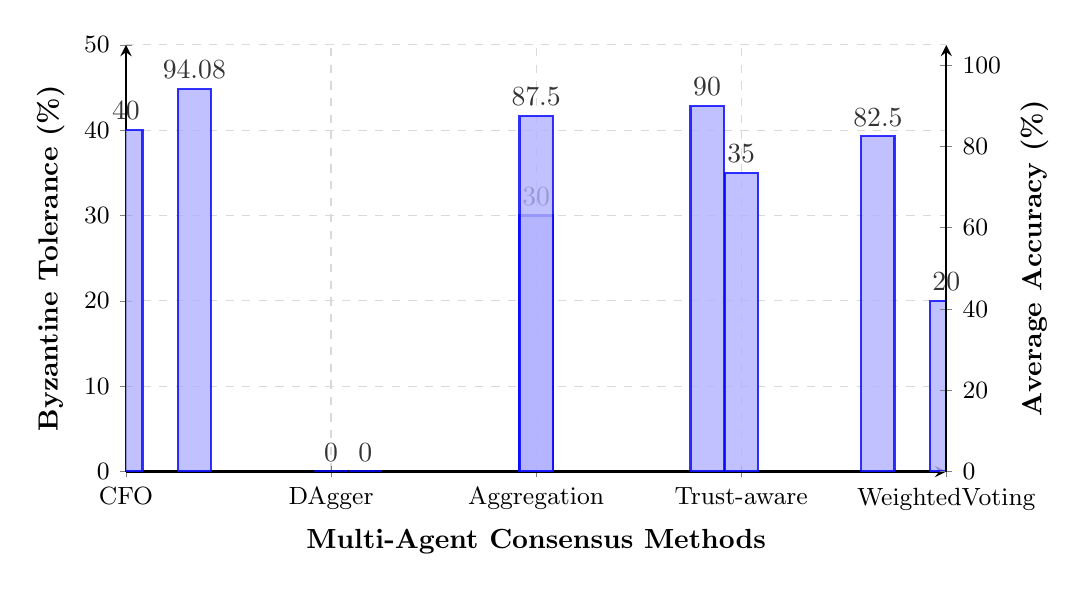
\begin{tikzpicture}
\begin{axis}[
    width=12cm,
    height=7cm,
    ybar=5pt,
    bar width=12pt,
    symbolic x coords={CFO,DAgger,Aggregation,Trust-aware,Weighted\\Voting},
    xtick=data,
    ylabel={Byzantine Tolerance (\%)},
    xlabel={Multi-Agent Consensus Methods},
    ymin=0, ymax=50,
    grid=both,
    grid style={dashed, gray!30},
    axis lines=left,
    axis line style={thick},
    every axis plot/.append style={fill=cfoBlue, opacity=0.8},
    nodes near coords,
    nodes near coords align={above},
    every node near coord/.append style={font=\bfseries, color=black}
]

\addplot coordinates {
    (CFO,40)
    (DAgger,0)
    (Aggregation,30)
    (Trust-aware,35)
    (Weighted\\Voting,20)
};

\end{axis}

\begin{axis}[
    width=12cm,
    height=7cm,
    ybar=5pt,
    bar width=12pt,
    symbolic x coords={CFO,DAgger,Aggregation,Trust-aware,Weighted\\Voting},
    xtick=data,
    ylabel={Average Accuracy (\%)},
    ymin=0, ymax=105,
    axis y line=right,
    axis x line=none,
    every axis plot/.append style={fill=krumOrange, opacity=0.8},
    nodes near coords,
    nodes near coords align={above},
    every node near coord/.append style={font=\bfseries, color=black}
]

\addplot coordinates {
    (CFO,94.08)
    (DAgger,0)
    (Aggregation,87.5)
    (Trust-aware,90)
    (Weighted\\Voting,82.5)
};

\end{axis}
\end{tikzpicture}
\caption{Comparison with Multi-Agent Consensus Methods}
\end{figure}

% Figure 4: Tolerance-Accuracy Trend
\begin{figure}[H]
\centering
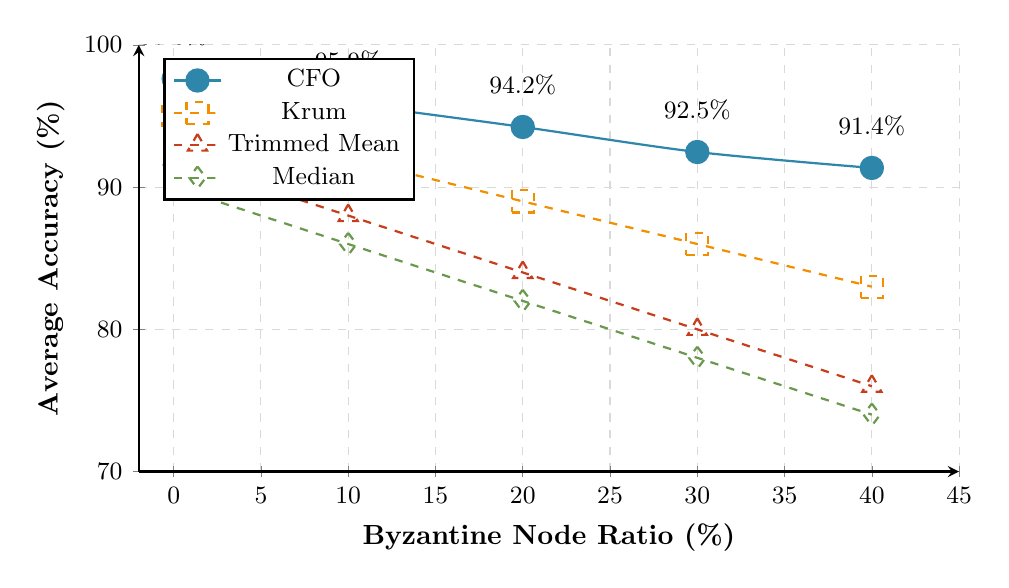
\begin{tikzpicture}
\begin{axis}[
    width=12cm,
    height=7cm,
    xlabel={Byzantine Node Ratio (\%)},
    ylabel={Average Accuracy (\%)},
    xmin=-2, xmax=45,
    ymin=70, ymax=100,
    grid=both,
    grid style={dashed, gray!30},
    axis lines=left,
    axis line style={thick},
    legend pos=north west,
    thick
]

\addplot[
    color=cfoBlue,
    mark=*,
    mark size=4pt,
    thick,
    smooth
] coordinates {
    (0,97.62)
    (10,95.88)
    (20,94.23)
    (30,92.47)
    (40,91.35)
};
\addlegendentry{CFO}

\addplot[
    color=krumOrange,
    mark=square,
    mark size=4pt,
    dashed,
    smooth
] coordinates {
    (0,95)
    (10,92)
    (20,89)
    (30,86)
    (40,83)
};
\addlegendentry{Krum}

\addplot[
    color=trimmedRed,
    mark=triangle,
    mark size=4pt,
    dashed,
    smooth
] coordinates {
    (0,92)
    (10,88)
    (20,84)
    (30,80)
    (40,76)
};
\addlegendentry{Trimmed Mean}

\addplot[
    color=medianGreen,
    mark=diamond,
    mark size=4pt,
    dashed,
    smooth
] coordinates {
    (0,90)
    (10,86)
    (20,82)
    (30,78)
    (40,74)
};
\addlegendentry{Median}

\node at (axis cs:0,97.62) [above=8pt] {97.6\%};
\node at (axis cs:10,95.88) [above=8pt] {95.9\%};
\node at (axis cs:20,94.23) [above=8pt] {94.2\%};
\node at (axis cs:30,92.47) [above=8pt] {92.5\%};
\node at (axis cs:40,91.35) [above=8pt] {91.4\%};

\end{axis}
\end{tikzpicture}
\caption{Relationship between Byzantine Tolerance and Prediction Accuracy}
\end{figure}

\end{document}